\documentclass[../../../../main.tex]{subfiles}
\begin{document}

\begin{flushright}
\footnotesize\textit{【自動文字起こし・要確認】}
\end{flushright}

[解] 外心から下ろした垂足は各辺の中点になっているから
Oを原点とする各点の位置ベクトルをその小文字で表すと
\begin{align*}
\vec{p} &= \frac{1}{2}(\vec{b} + \vec{c}) \\
\vec{q} &= \frac{1}{2}(\vec{a} + \vec{c}) \\
\vec{r} &= \frac{1}{2}(\vec{a} + \vec{b})
\end{align*}
これを等式に代入して
\begin{align*}
\frac{1}{2}(\vec{b} + \vec{c}) + \frac{2}{2}(\vec{a} + \vec{c}) + \frac{3}{2}(\vec{a} + \vec{b}) &= 0 \\
5\vec{a} + 4\vec{b} + 3\vec{c} &= 0 \quad \cdots \text{\textcircled{1}}
\end{align*}
である。変形して
\begin{equation*}
\vec{AO} = \frac{4\vec{AB} + 3\vec{AC}}{12}
\end{equation*}
$AB=k, AC=m$, $\vec{AB}$と$\vec{AC}$のなす角$\theta\ (0 < k, m, 0 < \theta < \pi)$として
*から
\begin{equation*}
\begin{cases}
\vec{AB} \cdot \left(\vec{AO} - \frac{1}{2}\vec{AB}\right) = 0 \\
\vec{AC} \cdot \left(\vec{AO} - \frac{1}{2}\vec{AC}\right) = 0
\end{cases}
\therefore \begin{cases}
-2k + 3m \cos\theta = 0 \quad \cdots \text{\textcircled{2}} \\
-3m + 4k \cos\theta = 0 \quad \cdots \text{\textcircled{3}}
\end{cases}
\end{equation*}
\textcircled{2}から $k = \frac{3}{2}m \cos\theta$ だから、\textcircled{3}に代入して $\cos^2\theta = \frac{1}{2} \ (\because m \neq 0)$ \\
$k > 0, m > 0$ から $\cos\theta > 0$ で、$\cos\theta = \frac{\sqrt{2}}{2} \quad \therefore \angle BAC = \frac{\pi}{4}$ である。

[別 - 円周角を考えて...]
\textcircled{1}から $\vec{a}$ を消去して $\vec{b} \cdot \vec{c} = 0$ がすぐ求まるが。

\begin{center}
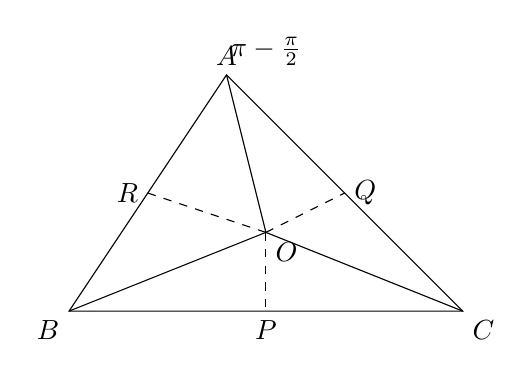
\begin{tikzpicture}
\coordinate (A) at (0,3);
\coordinate (B) at (-2,0);
\coordinate (C) at (3,0);
\coordinate (O) at (0.5,1);
\coordinate (P) at (0.5,0);
\coordinate (Q) at (1.5,1.5);
\coordinate (R) at (-1,1.5);

\draw (A) node[above] {$A$} -- (B) node[below left] {$B$} -- (C) node[below right] {$C$} -- cycle;
\draw[dashed] (O) node[below right] {$O$} -- (P) node[below] {$P$};
\draw[dashed] (O) -- (Q) node[right] {$Q$};
\draw[dashed] (O) -- (R) node[left] {$R$};
\draw (A) -- (O);
\draw (B) -- (O);
\draw (C) -- (O);

\node at (0.5,3.3) {$\pi - \frac{\pi}{2}$};
\end{tikzpicture}
\end{center}

\end{document}
